\documentclass{hnnuthesis}

%%%%%%%%%%%%%%%%%%%%%%%%%%%%%%%%%%%%
% 填写论文信息
%%%%%%%%%%%%%%%%%%%%%%%%%%%%%%%%%%%%

\titleinfo
{基于 RISC-V 架构的处理器设计与实现}
{张吼吼}
{224456634560}
{2022级计科8班}
{计算机学院}
{唐教授}

\secondsupervisorinfo{李教授}
\thesisdate{2026}{6}[18]

\begin{document}

%%%%%%%%%%%%%%%%%%%%%%%%%%%%%%%%%%%%
% 封面
%%%%%%%%%%%%%%%%%%%%%%%%%%%%%%%%%%%%

\makethesistitle

%%%%%%%%%%%%%%%%%%%%%%%%%%%%%%%%%%%%
% 中文摘要
%%%%%%%%%%%%%%%%%%%%%%%%%%%%%%%%%%%%

\cabstract
{本文以基于 RISC-V 架构的处理器设计为研究对象，围绕指令系统、数据通路、控制器设计以及功能验证等内容展开分析。首先介绍课题研究背景与意义，其次对处理器总体结构与关键模块实现方法进行阐述，最后结合实验结果对系统性能与正确性进行验证。研究结果表明，该设计能够较好地完成基本指令执行任务，并满足本科毕业设计（论文）写作与排版要求。

本文同时给出模板中封面、摘要、目录、章节、图表、公式、参考文献、致谢及附录等命令的使用示例，便于直接参考与修改。}
{RISC-V；处理器设计；数据通路；控制器；功能验证}

%%%%%%%%%%%%%%%%%%%%%%%%%%%%%%%%%%%%
% 英文摘要
%%%%%%%%%%%%%%%%%%%%%%%%%%%%%%%%%%%%

\eabstract
{Design and Implementation of a Processor Based on RISC-V Architecture}
{This thesis focuses on the design and implementation of a processor based on the RISC-V architecture. It discusses the instruction set, datapath, control unit, and functional verification. The background and significance of the topic are introduced first, then the overall structure and key modules are analyzed, and finally experimental results are used to verify the correctness and effectiveness of the design.

This sample also demonstrates how to use the cover page, abstract, table of contents, headings, figures, tables, equations, references, acknowledgments, and appendix commands defined in the thesis class.}
{RISC-V; processor design; datapath; control unit; verification}

%%%%%%%%%%%%%%%%%%%%%%%%%%%%%%%%%%%%
% 目录
%%%%%%%%%%%%%%%%%%%%%%%%%%%%%%%%%%%%

\tableofcontents

%%%%%%%%%%%%%%%%%%%%%%%%%%%%%%%%%%%%
% 正文
%%%%%%%%%%%%%%%%%%%%%%%%%%%%%%%%%%%%

\startmain

\section{绪论}

\subsection{课题背景及目的}

随着开源芯片生态的快速发展，RISC-V 架构因其开放、精简和可扩展等特点，逐渐成为处理器设计领域的重要研究方向。围绕 RISC-V 架构开展本科毕业设计，不仅有助于理解计算机组成原理、数字逻辑与硬件描述语言等核心课程内容，也能够提升系统设计与综合实践能力\upcite{ref2}。

本课题旨在完成一个基础处理器系统的设计与验证，通过对指令译码、寄存器堆、算术逻辑单元及控制模块的分析，实现基本指令的正确执行，并为后续功能扩展提供实验基础。这里同时演示正文首段缩进和参考文献引用格式，例如也可以直接写作\cite{ref1}。

\subsection{国内外研究状况}

近年来，国内外高校与研究机构围绕 RISC-V 指令集开展了大量研究。国外研究更关注高性能内核、编译工具链与生态建设，国内研究则在教学实验平台、嵌入式控制与国产化替代等方面取得了明显进展。总体来看，RISC-V 已具备良好的教学与工程应用价值。

\section{层级叶/盘转子错频方案的对比分析}

\subsection{基础知识}

在叶轮机械领域，对一个实际的叶盘转子，错频是指由于单个叶片之间因几何上或结构上的不同而造成的其在固有频率上的差异\upcite{ref1}。为了分析不同错频方案对系统振动特性的影响，通常需要从结构参数、动力学方程及响应特征等多个角度展开研究。

由前面的分析可知，建立合理的动力学模型是后续响应分析的基础。正文在节标题之后的首段现在也会自动首行缩进两个字，不需要手动补空格。

公式示例如下：

\begin{equation}
C = A + B
\end{equation}

若公式较长，可采用多行公式环境，并尽量在等号或运算符处换行：

\begin{align}
F(x) &= x_1 + x_2 + x_3 + x_4 \\
     &\quad + x_5 + x_6 + x_7
\end{align}

\subsection{多自由度系统的强迫响应分析}

由前面的分析可知，响应分析在数学上通常需要求解多自由度系统在外激励作用下的稳态响应与瞬态响应。通过建立质量矩阵、阻尼矩阵和刚度矩阵，可以进一步讨论不同错频参数对振动幅值和共振区间的影响。

在关键模块设计或理论分析中，若需要分项论述，可直接使用枚举环境，模板会自动显示为全角序号：

\begin{enumerate}
    \item 建立系统动力学模型；
    \item 分析不同参数下的固有频率变化；
    \item 比较不同错频方案的响应差异。
\end{enumerate}

图示例如下：

\begin{figure}[h]
\centering
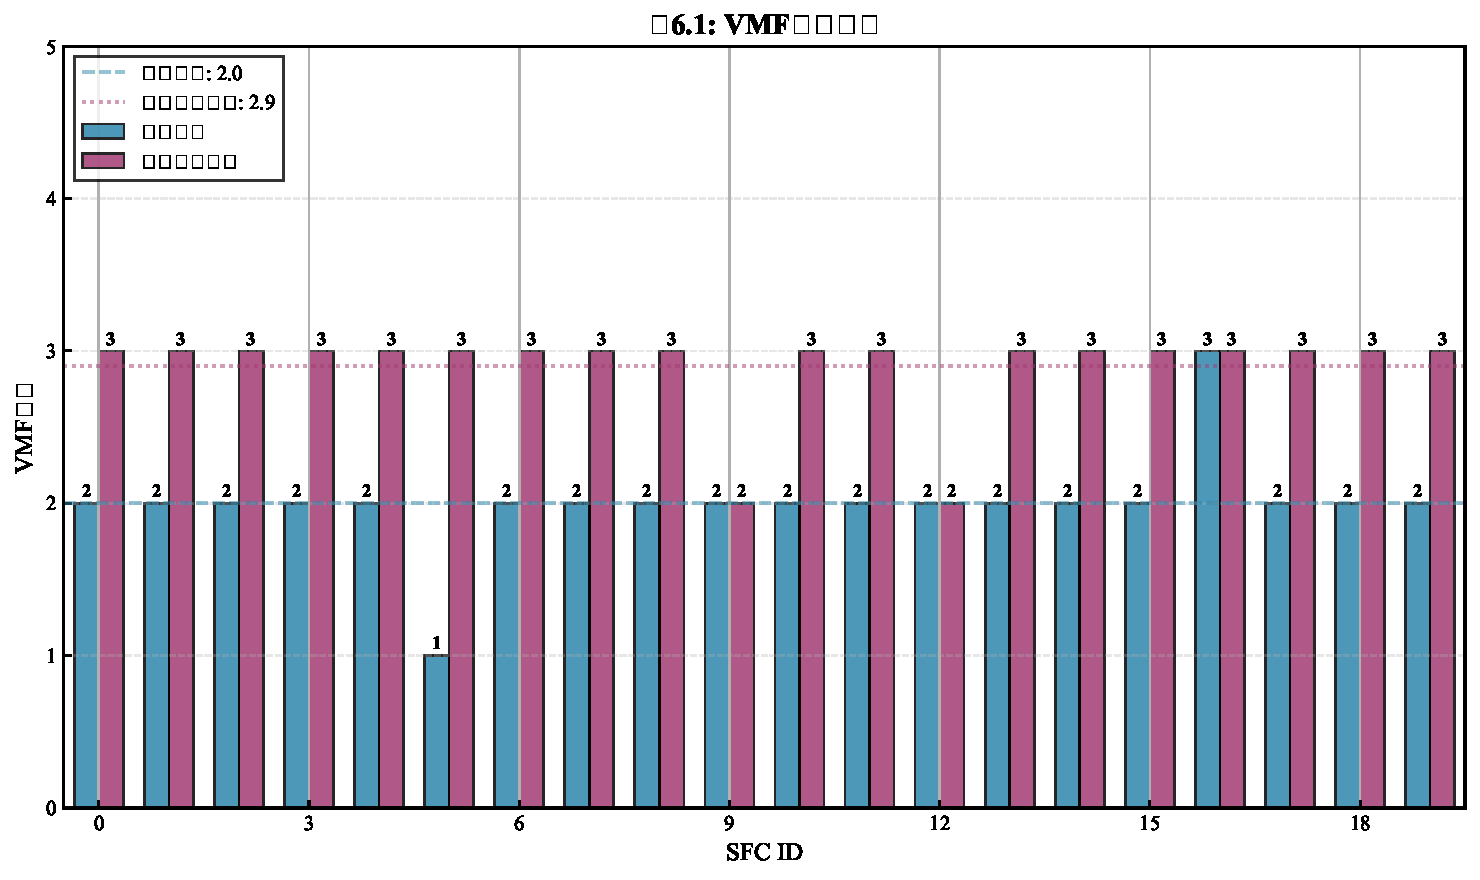
\includegraphics[width=0.55\textwidth]{example.pdf}
\caption{示例矢量图插入效果}
\label{fig:cpu-arch}
\end{figure}

可在正文中引用图 \ref{fig:cpu-arch}，也可结合表 \ref{tab:function} 进行说明。

表格示例如下：

\begin{table}[h]
\centering
\caption{关键模块功能说明}
\label{tab:function}
\begin{tabular}{ccc}
\toprule
编号 & 模块名称 & 功能说明\\
\midrule
1 & 控制器 & 生成控制信号\\
2 & ALU & 完成算术逻辑运算\\
3 & 寄存器堆 & 暂存运算数据\\
\bottomrule
\end{tabular}
\end{table}

\subsection{小结}

本章从理论背景、公式、图表、分项序号与文献引用等方面给出了完整示例，可直接作为模板使用参考。

\section{结论}

本文完成了基于 RISC-V 架构的基础处理器设计示例，并给出了 `hnnuthesis.cls` 中主要命令的使用方法，包括 `\titleinfo`、`\secondsupervisorinfo`、`\thesisdate`、`\makethesistitle`、`\cabstract`、`\eabstract`、`\startmain`、`\acknowledgment` 与 `\appendixpage` 等，可作为湖南第一师范学院本科毕业设计（论文）的排版示例。

%%%%%%%%%%%%%%%%%%%%%%%%%%%%%%%%%%%%
% 参考文献
%%%%%%%%%%%%%%%%%%%%%%%%%%%%%%%%%%%%

\begin{thebibliography}{99}

\bibitem{ref1}
刘国钧．图书馆史研究[M]．北京：高等教育出版社，1979．

\bibitem{ref2}
Patterson D A, Hennessy J L. Computer Organization and Design[M]. San Francisco: Morgan Kaufmann, 2017.

\end{thebibliography}

%%%%%%%%%%%%%%%%%%%%%%%%%%%%%%%%%%%%
% 致谢
%%%%%%%%%%%%%%%%%%%%%%%%%%%%%%%%%%%%

\acknowledgment{在本论文撰写过程中，感谢指导教师与第二导师在选题、设计和写作过程中给予的帮助与支持，感谢同学与家人在学习和生活中的鼓励。本段展示了致谢命令的直接用法。}

%%%%%%%%%%%%%%%%%%%%%%%%%%%%%%%%%%%%
% 附录
%%%%%%%%%%%%%%%%%%%%%%%%%%%%%%%%%%%%

\appendixpage

\section{程序代码}

下面给出附录命令与代码展示环境的示例：

\begin{verbatim}
module alu(
    input  [31:0] a,
    input  [31:0] b,
    input  [2:0]  alu_op,
    output [31:0] y
);
endmodule
\end{verbatim}

\end{document}
